% ==============================================================================
% LQ CONTROL
% ==============================================================================

\begin{frame}{LQ control}
    \framesubtitle{Linear-quadratic control design}

    \begin{columns}[T,onlytextwidth]
        \begin{column}{0.48\textwidth}
            \begin{block}{Control principle}
                \centering
                \begin{tikzpicture}[
                    auto,
                    >=Stealth,
                    thick,
                    node distance=1.2cm,
                    block/.style={
                        draw,
                        rectangle,
                        align=center,
                        minimum height=0.8cm,
                        minimum width=1.55cm,
                        inner sep=2pt,
                        fill=blue!5,
                        rounded corners=2pt,
                        font=\scriptsize
                    }
                ]
                    \node (reference) {};
                    \node[block, right=of reference] (lqr) {\textbf{LQ}\\[-1pt]\tiny Linear model};
                    \node[block, right=of lqr] (system) {\textbf{System}\\[-1pt]\tiny (Drone)};
                    \node[right=0.55cm of system] (output) {};

                    \draw[->] (reference) -- node {$r$} (lqr);
                    \draw[->] (lqr) -- node {$u$} (system);
                    \draw[->] (system) -- node {$a_z$} (output);
                \end{tikzpicture}
            \end{block}

            \begin{exampleblock}{Performance}
                \begin{itemize}
                    \item Global trajectory following
                    \item Wrong amplitude + phase shift
                    \item Missing prediction
                \end{itemize}
            \end{exampleblock}
        \end{column}

        \begin{column}{0.48\textwidth}
            \centering
            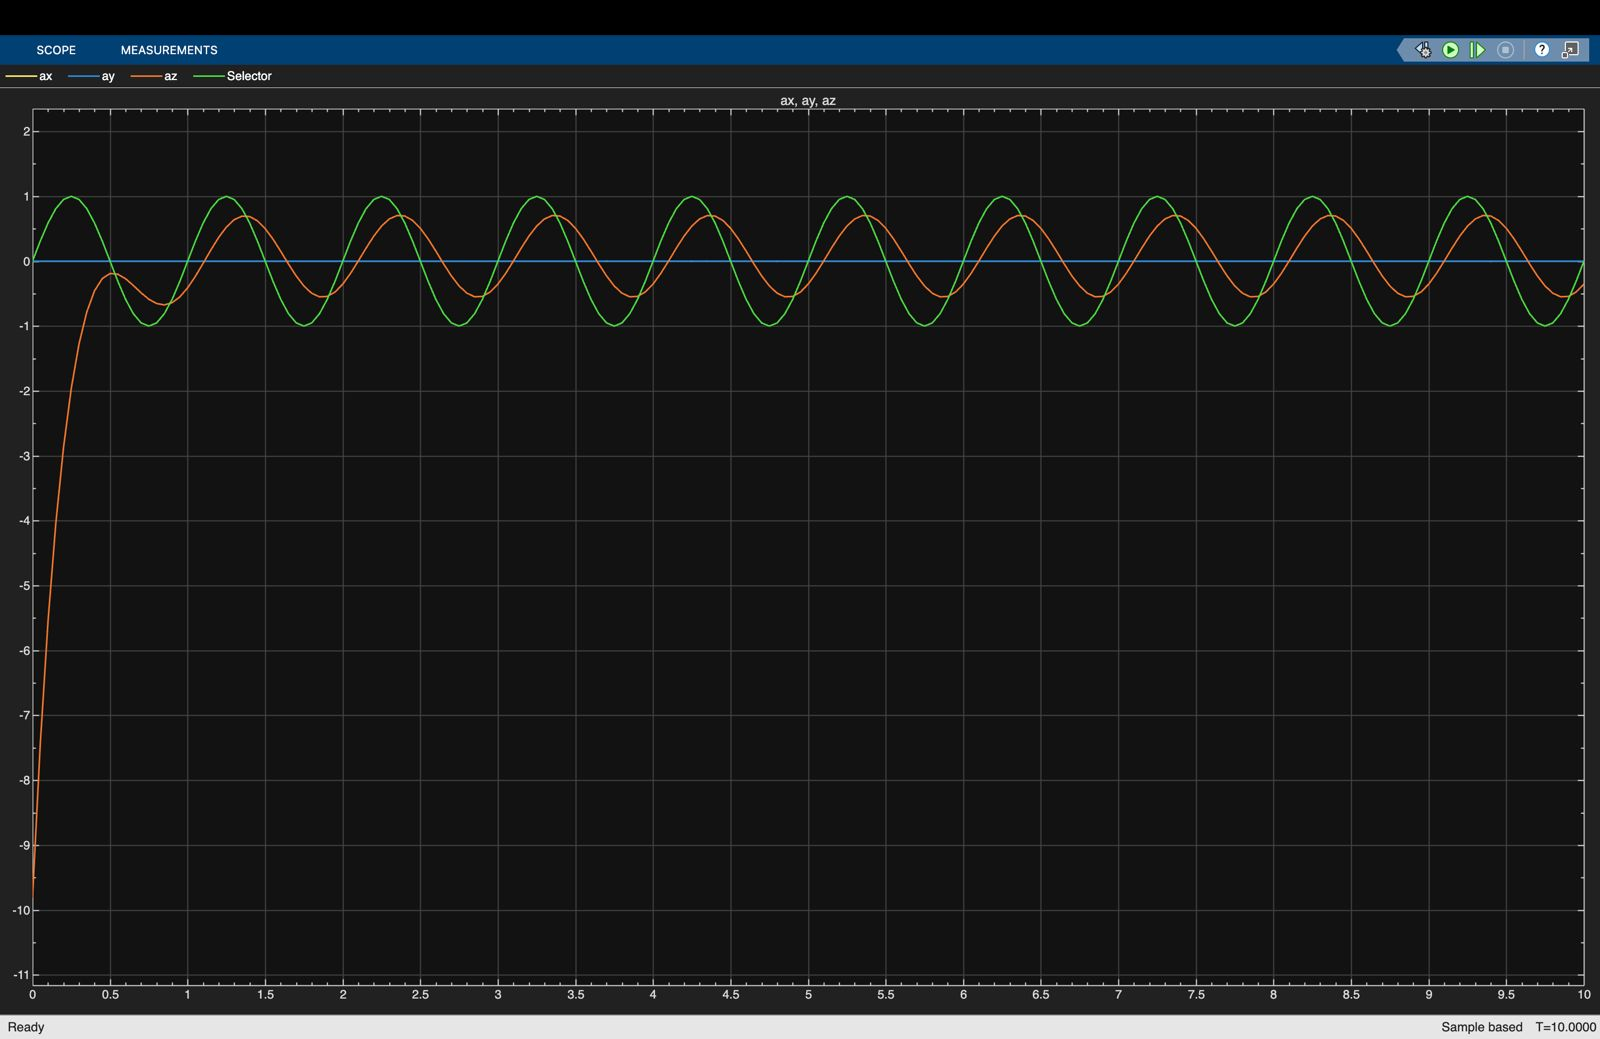
\includegraphics[
                width=\linewidth,
                height=5.5cm,
                keepaspectratio
            ]{lqr_linear_sinewave.jpeg}
        \end{column}
    \end{columns}
\end{frame}
